\chapter{Process}

\section{Process Concept}

\textbf{Process} is a program in execution. Process execution must progress in sequential fashion, there are not parallel execution of instructions of a single process. 
\paragraph{}
Program is \textbf{passive} entity stored on disk (executable file), process is \textbf{active} so program becomes process when an executable file is loaded into memory.

One program can be has several process, think about multiple users executing.

\paragraph{}
An OS executes a variety of programs:
\begin{itemize}
    \item Batch system – jobs
    \item Time-shared systems – user programs or tasks
\end{itemize}

\paragraph{}
Process has multiple parts:
\begin{itemize}
    \item The program code, called text section
    \item Current activity including PC, processor register
    \item Stack containing temporary data (function params, return addresses, local variables)
    \item Data section containing global variables
    \item heap containing memory dynamically allocated during run time
\end{itemize}

\subsubsection{Memory layout of a C program}

\begin{figure}[htbp]
    \centering
    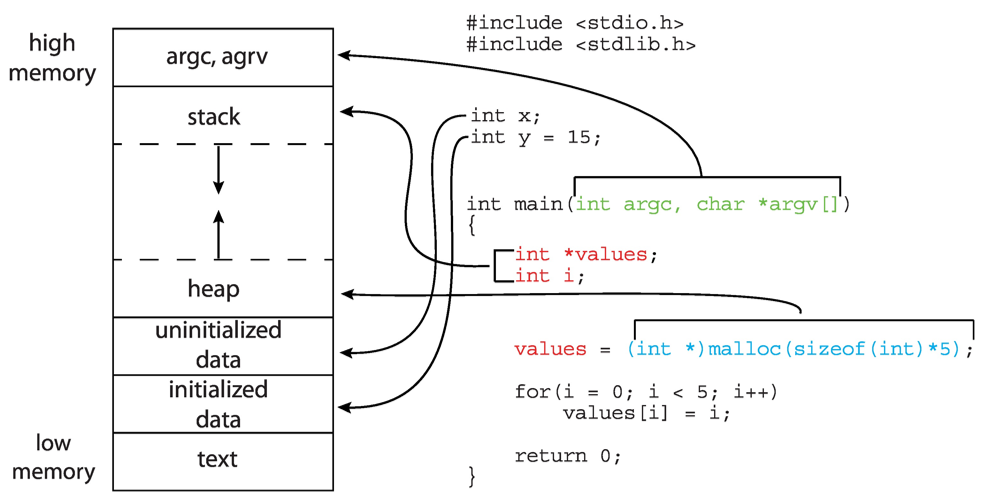
\includegraphics[width=0.7\linewidth]{img/memory_c_program.png}
    \caption{Relation to C program and memory usage}    
\end{figure}

We see that the heap grows upwards and the stack vice versa, this structure is used for efficiency. 

\subsection{Process State}
Process during this life change it states:

\begin{itemize}
    \item \textbf{New:} The process is being created
    \item \textbf{Ready:} The process is waiting to be assigned to a processor
    \item \textbf{Running:} Instruction are being executed
    \item \textbf{Waiting:} Process waiting for some event to occur (mouse click, I/O, interrupt)    
    \item \textbf{Terminated:} The process has finished execution
\end{itemize}


\begin{figure}[htbp]
    \centering
    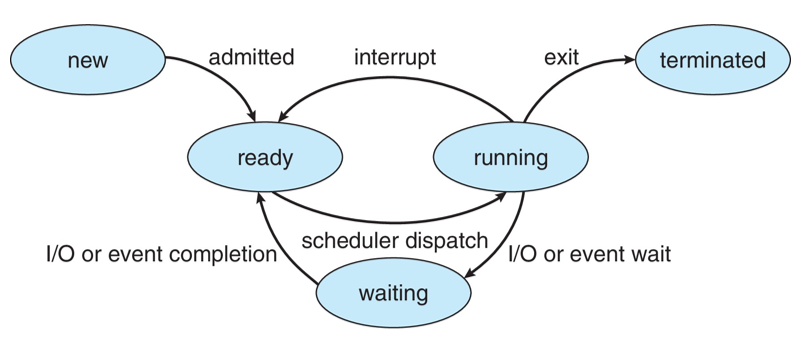
\includegraphics[width=0.6\linewidth]{img/process_state_diagram.png}
    \caption{Diagram of Process State}    
\end{figure}

\section{Process Control Block (PCB)}
All process must have information about the state, this block of information is called PCB and contains:

\begin{itemize}
    \item Process state - running, waiting...
    \item Program counter - location to the next code to execute
    \item CPU register 
    \item CPU scheduling info - priorities, scheduling queue
    \item Memory-management info - memory allocated to the process
    \item Accounting info - CPU usage, time since start, time limits
    \item I/O status info - list of open files
\end{itemize}

All of this information are used because when i resume the process i want the same data loaded into register and cache.

\begin{figure}[htbp]
    \centering
    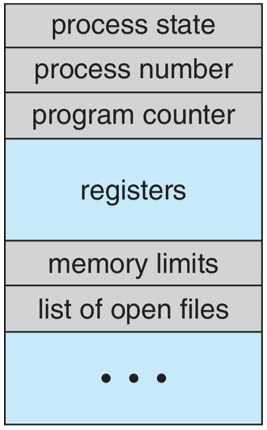
\includegraphics[width=0.17\linewidth]{img/PCB.png}
    \caption{Process Control Block (PCB)}    
\end{figure}

In Ubuntu we see PCBs in the folder: \verb|cat /proc/self/status| in this way we see the PCB of cat call, if we replace self with 1 (PID), we see the PCB of systemd.
Or using top command to see all Process ID.



\subsection{Context Switching}

When process require to wait, CPU stops to work on it an pass to another task. When CPU switch to another process, the system must save the state of the old process and load the salved state for the new process via \textbf{context switch}. The context is represented in the PCB.

Context switching time is pure overhead; the system does no useful work while switching, it is just a waste of time. More complex are OS and PCB and more longer context switch.

\section{Threads}
First of all threads are different from process, because if P1 run only one task it is a single thread process, otherwise is P1 run more tasks it becomes multi-thread process.
\paragraph{}
So far, a process has a single "script" of function, but now I want to code a program to execute in parallel to implement parallel search ecc. 

How can I do it?
\paragraph{}
Each thread has a PC assigned, thus a process has multiple program counter (Multiple locations can execute at once).

\begin{figure}[htbp]
    \centering
    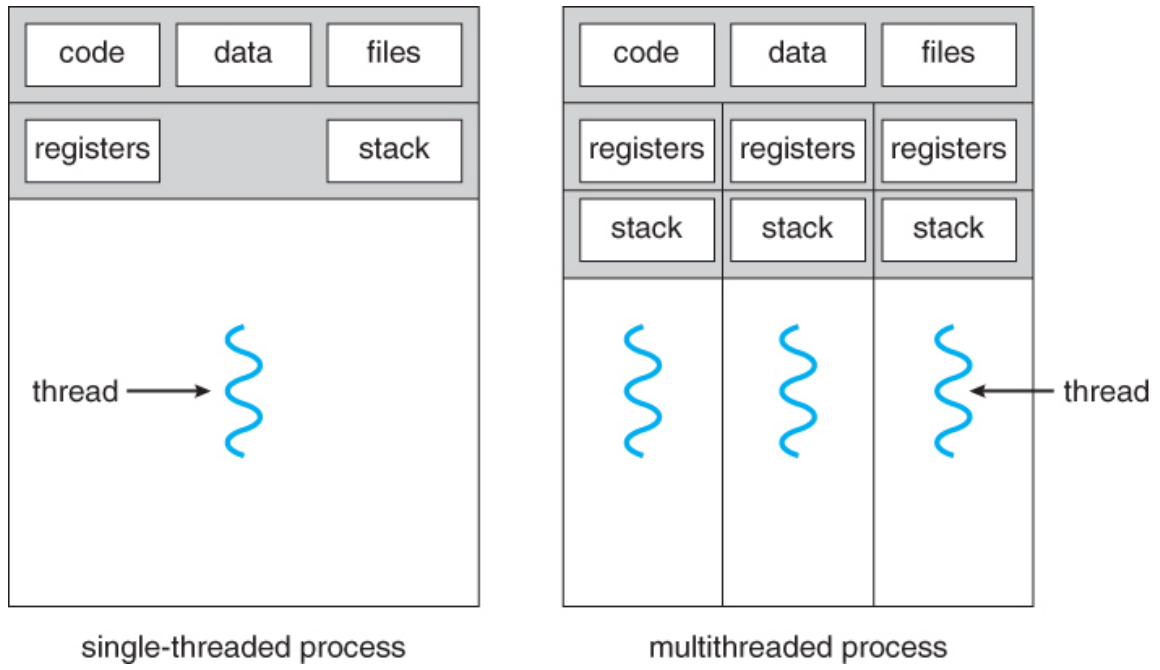
\includegraphics[width=0.5\linewidth]{img/thread.png}    
\end{figure}


\subsection{Multitasking in Mobile System}
Some mobile systems (e.g., early version of iOS)  allow only one process to run, others suspended.

\paragraph{IOS:}

\begin{itemize}
    \item Single foreground process- controlled via user interface
    \item Multiple background processes– in memory, running, but not on the display, and with limits
    \item Limits include single, short task, receiving notification of events, specific long-running tasks like audio playback

\end{itemize}


\paragraph{Android runs foreground and background, with fewre limits:}

\begin{itemize}
    \item Background process uses a service to perform tasks
    \item Service can keep running even if background process is suspended
    \item Service has no user interface, small memory use
\end{itemize}


\newpage
\section{Process Scheduling}

Process scheduler selects among available process for next execution on CPU core, the main goal of this process is to maximize the use of CPU, quickly switching onto CPU core.
Maintains updated two queue:

\begin{itemize}
    \item Ready queue: for all process that are ready to being execute
    \item Wait queues: for process that wait for some events (I/O)
\end{itemize}
Process normally migrate from one queue to the other.

\begin{figure}[htbp]
    \centering
    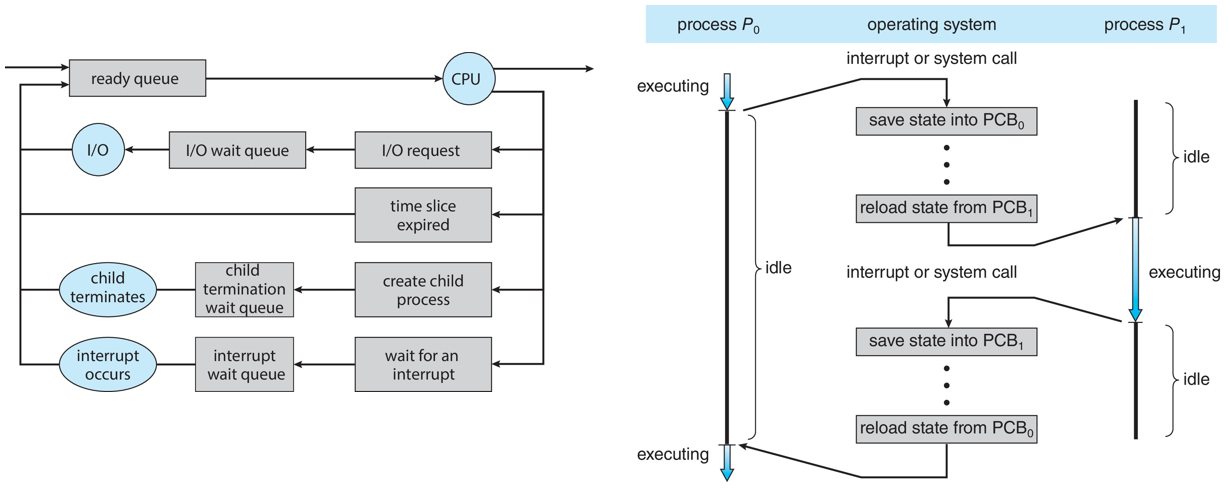
\includegraphics[width=0.95\linewidth]{img/scheduling.png}
    \caption{Process scheduling left; CPU switching right}    
\end{figure}



\section{Process Creation: }
Parent process create children process, witch can create other processes, forming a tree of processes.

Each process is \textbf{identified} by a process identifier: \textbf{pid} and they also has \textbf{resources} that could be shared by sharing option:

\begin{itemize}
    \item Parent and children share all resources
    \item Children share subset of parent's resources, like C++ Inheritance
    \item Parent and child share no resources
\end{itemize}

Processes can decide how to \textbf{execute}: parent and children execute concurrently or parent waits until children terminate.

Address space: 
\begin{itemize}
    \item Child duplicate of parent
    \item Child has a program loaded into it
\end{itemize}

\paragraph{UNIX example of OS-call:}
\begin{itemize}
    \item \textbf{fork()} : to create new process, return a $pid_t$ of children created
    \item \textbf{exec()} : used after fork() to replace the process' memory space with new program
    \item \textbf{wait()} : used by parent to waiting for the child to terminate.
\end{itemize}


\begin{figure}[htbp]
    \centering
    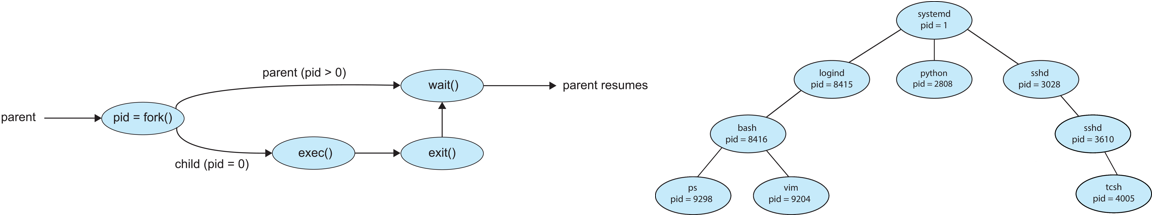
\includegraphics[width=1\linewidth]{img/process.png}
    \caption{OS-call left; process tree in Linux, \textit{pstree command}}    
\end{figure}


\subsubsection{C program forking separate process}
\begin{codeInC}
#include <sys/types.h>
#include <stdio.h>
#include <unistd.h>

int main() {

  pid_t pid;

  /* fork a child process */
  pid = fork();

  if (pid < 0) { /* error occurred */
    fprintf(stderr, "Fork Failed");
    return 1;
  } else if (pid == 0) { /* child process */
    execlp("/bin/ls", "ls", NULL);

  } else { /* parent process */

    /* parent will wait for the child to complete */
    wait(NULL);
    printf("Child Complete");
  }  

  return 0;
}

\end{codeInC}


\newpage
\section{Process termination}

Each process can decide to terminate the task at any time. Process usually executes last statement and than asks to the OS to delete it using \textbf{ exit()} call.

All children's status returns to parent (via \textbf{wait()} call) and process' resources are deallocated by OS.

In some cases parent can use the \textbf{abort()} call to terminate the execution of children. Some reasons of doing it:

\begin{itemize}
    \item Children has exceeded allocated resources
    \item The task assigned to children is no longer required
    \item OS call exit() call to the parent process and children must terminate to do the assigned task because OS does not allow to continue if its parent terminates.
\end{itemize}

Some OS wait until all the process terminates' children terminates, it called cascading termination.
The parent process may wait for termination of a child process by using \textbf{wait() syscall}. The call returns status, information and pid of the terminated process.

\begin{codeInC}
pid  = wait(&status);
\end{codeInC}

If no parent waiting (did not invoke wait()) process is a \textbf{zombie}.

If parent terminated without invoking wait(), process is an \textbf{orphan}.



\section{Android process termination importance hierarchy}
All mobile smartphones have limited resources such as memory compare to PCs. Thus, the android OS has to manage process termination to improve performance. Below there is a list of process, from most to least important: 

\begin{itemize}
    \item Foreground process;
    \item Visible process;
    \item Service process;
    \item Background process;
    \item Empty process;
\end{itemize}

Android terminates less important processes weed out unused memory. 

\section{Inter-process Communication}

Process within a system may be \textbf{independent} or \textbf{cooperating}.
Cooperating process can affect or be affected by other processes, including sharing data.

Cooperating processes need \textbf{interprocess communication} \textbf{IPC}, obviously there are reasons for cooperating process:

\begin{itemize}
    \item information sharing;
    \item computation speedup;
    \item modularity;
    \item convenience;
\end{itemize}

\paragraph{}
Also there are two different way to implement IPC: 
\begin{itemize}
    \item Shared memory: you define a specific space into ram where two process can access and communicate
    \item Message passing
\end{itemize}

\begin{figure}[htbp]
    \centering
    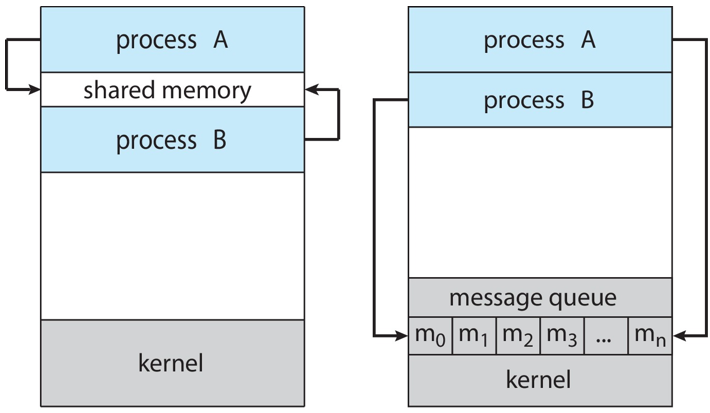
\includegraphics[width=0.5\linewidth]{img/IPC.png}
    \caption{shared memory left; message passing right}    
\end{figure}

\subsection{Producer-consumer problem}

Producer process produces information that is consumed by consumer process, two variations:

\begin{itemize}
    \item unbounded-buffer places no practical limit on the size of buffer:
    \begin{itemize}
        \item[] Producer never waits
        \item[] consumer waits if there is no buffer to consume
    \end{itemize}

    \item bounded-buffer assumes that there is a fixed buffer size:
    \begin{itemize}
        \item[] Producer must wait if all buffer are full
        \item[] Consumer waits if there is no buffer to consume
    \end{itemize}
\end{itemize}

 \subsection{IPC - Message Passing}
Major issues is to provide mechanism that will allow the user processes to synchronize their actions when they access shared memory.

\subsubsection{Example of IPC - POSIX}
POSIX Shared Memory: Process P1 create shared memory segment, an area of RAM memory.

\begin{codeInC}
shm_fd = shm_open(name, O CREAT | O RDWR, 0666);
\end{codeInC}

and set the size of the existing segment:
\begin{codeInC}
ftruncate(shm_fd, 4096); 
\end{codeInC}

In this way you create an area of memory and you must use it like a file, calling the default call for file descriptor: open, read, write, close, seek...

\newpage
\subsubsection{Memory-map}
If you use the function \textit{mmap()}, you transform the file in array of bytes. You just modified the access to the byets not the content. Using this method you also can access to virtual memory a concept that we will see later.


\subsubsection{IPC POSIX Producer}
\begin{codeInC}
#include <stdio.h>
#include <stdlib.h>

#include <string.h>
#include <fcntl.h>

#include <sys/shm.h>
#include <sys/stat.h>

int main() {

    /* the size (in bytes) of shared memory object */
    const int SIZE = 4096;
    
    /* name of the shared memory object */
    const char *name = "OS";
    
    /* strings written to shared memory */
    const char *message0 = "Hello";
    const char *message1 = "World!";
    
    /* shared memory file descriptor */
    int shm_fd;
    
    /* pointer to shared memory object */
    void *ptr;
    
    /* create the shared memory object */
    shm_fd = shm_open(name, O_CREAT | O_RDWR, 0666);
    
    /* configure the size of the shared memory object */
    ftruncate(shm_fd, SIZE);
    
    /* memory map the shared memory object */
    ptr = mmap(0, SIZE, PROT_WRITE, MAP_SHARED, shm_fd, 0);
    
    /* write to the shared memory object */
    sprintf(ptr, "%s", message0);    
    ptr += strlen(message0);  // you must do it otherwise you rewrite the bytes
    sprintf(ptr, "%s", message1);
    ptr += strlen(message1);
    
    return 0;
}

\end{codeInC}

\newpage
\subsubsection{IPC POSIX Consumer}
\begin{codeInC}
#include <stdio.h>
#include <stdlib.h>

#include <fcntl.h>
#include <sys/shm.h>

#include <sys/stat.h>

int main() {

    /* the size (in bytes) of shared memory object */
    const int SIZE = 4096;
    
    /* name of the shared memory object */
    const char *name = "OS";
    
    /* shared memory file descriptor */
    int shm_fd;
    
    /* pointer to shared memory object */
    void *ptr;
    
    /* open the shared memory object */
    shm_fd = shm_open(name, O_RDONLY, 0666);
    
    /* memory map the shared memory object */
    ptr = mmap(0, SIZE, PROT_READ, MAP_SHARED, shm_fd, 0);
    
    /* read from the shared memory object */
    printf("%s", (char *)ptr);    
    
    /* remove the shared memory object */
    shm_unlink(name);  //like close(), you free the memory to OS.
    
    return 0;
}

\end{codeInC}


The only way to get access the S.M. is to know the name of the shared memory object, so it must be \textbf{secret}.

\newpage
 \subsection{IPC - Message Passing}
 Processes communicate with each other without resorting to shared variables, thus IPC provide two option: \textbf{send} and \textbf{receive} massage. The size of message is fixed or variable.

 \paragraph{}
 If process \textit{P} and \textit{Q} wish to communicate, they need:
 \begin{itemize}
     \item Establish a communication link between them
     \item Exchange messages via send and receive
 \end{itemize}
 
\paragraph{How to implement this communication?} How to establish the link? The link is connected with one ore more processes? Capacity of the link? 

\subsection{Direct Communication}
Processes must name each other explicitly:

\begin{itemize}
    \item send(P, msg) - send a message to process P
    \item receive(Q, msg) - receive a message from process Q
\end{itemize}

The proprieties of communication link are: links are established automatically, bi-directional and between each pair exist only one link.

\subsection{Indirect communication}

Indirect communication is different as Direct communication because it uses a mailbox to communicate.


Each mailbox has a unique id and process can communicate only if they share a mailbox.

The proprieties of communication link are: links are established only if processes share a common mailbox, link could be associated with several processes and each process may share several communication links, links may be unidirectional or bi-directional.

\begin{itemize}
    \item send(A, msg) - send a message to mailbox A
    \item receive(A, msg) - receive a message from mailbox A
\end{itemize}

In this way there is a problem. If P1, P2 and P3 share mailbox A and P1 send a message, who receive the message?

\paragraph{Some solutions could be:}
\begin{itemize}
    \item Create link associated only a two processes (like direct communication)
    \item  Allow only one process at a time to execute a receive operation
    \item Allow the system to select arbitrarily the receiver
\end{itemize}

\newpage
\subsection{Synchronization}
The messages could be blocking or non-blocking message:


\paragraph{Blocking} is considered synchronous
\begin{itemize}
    \item \textbf{Blocking send} - the sender is blocked until the message is received
    \item \textbf{Blocking receive} - the receiver is blocked until the message is available
\end{itemize}

\paragraph{Non-blocking} is considered asynchronous
\begin{itemize}
    \item \textbf{Non-blocking send} - the sender sends the message and continue
    \item \textbf{Non-blocking receive} - the receiver receives a valid message or null message
\end{itemize}

Different combinations are possible but if both, sender and receiver, are blocked we have a \textbf{rendezvous}.

\subsection{IPC Systems - Windows}

The message passing in Windows pass throw \textbf{advanced local procedure call}: 
\begin{itemize}
    \item Only works between processes on the same system
    \item Uses ports (like mailbox) to established and maintain communication link
\end{itemize}

Communication works as follows:

\begin{enumerate}
    \item The client open a handle to the subsystem's connection port object
    \item the client sends a connection request
    \item the server create two private communication ports and return the handle to the client
    \item the client and server use corresponding port handle to send messages and/or callback a to listen for replies
\end{enumerate}

\begin{figure}[htbp]
    \centering
    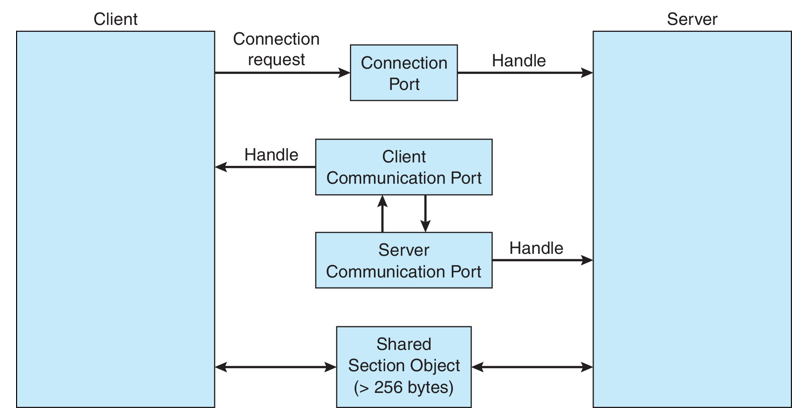
\includegraphics[width=0.65\linewidth]{img/LPC.png}
    \caption{Message passing via advanced Local Call LPO}
    
\end{figure}

\newpage
\section{Pipes}
Pipes acts as a conduit allowing to processes to communicate. There are some issues like: are uni or bi directional and in case of two-way communication it is half or full duplex?

There are two different type of pipes:

\begin{itemize}
    \item \textbf{Ordinary pipes} - the pipe cannot be accessed from outside the process that created it. Typical example might be: parent create a process and want to communicate with child that it created.
    \item \textbf{Named pipes} - can be accessed without a parent-child relationship
\end{itemize}

To create a pipe you must call the \textit{mkfifo("name", 0666)}

\subsection{Ordinary pipes}
This ordinary pipe allow to communicate only if you have a parent-child relationship.

Producer write in one end (write-end) and the consumer read from the another end (read-end). Ordinary pipes are therefore unidirectional.

\begin{figure}[htbp]
    \centering
    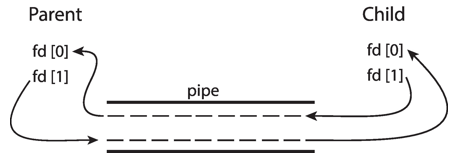
\includegraphics[width=0.55\linewidth]{img/O_Pipes.png}
    \caption{Ordinary pipes}    
\end{figure}

Windows calls this pipe \textbf{anonymous pipes}.

\newpage
\subsubsection{Ordinary UNIX pipes}
\begin{codeInC}
#include <stdio.h>
#include <unistd.h>
#include <sys/types.h>
#include <string.h>

#define BUFFER_SIZE 25
#define READ_END	0
#define WRITE_END	1

int main(void){
	char write_msg[BUFFER_SIZE] = "Greetings";
	char read_msg[BUFFER_SIZE];
	pid_t pid;
	int fd[2];

	/* create the pipe */
	if (pipe(fd) == -1) {
		fprintf(stderr,"Pipe failed");
		return 1;
	}

	/* now fork a child process */
	pid = fork();

	if (pid < 0) {
		fprintf(stderr, "Fork failed");
		return 1;
	}

	if (pid > 0) {  /* parent process */
		/* close the unused end of the pipe */
		close(fd[READ_END]);

		/* write to the pipe */
		write(fd[WRITE_END], write_msg, strlen(write_msg)+1); 

		/* close the write end of the pipe */
		close(fd[WRITE_END]);
	}
	else { /* child process */
		/* close the unused end of the pipe */
		close(fd[WRITE_END]);

		/* read from the pipe */
		read(fd[READ_END], read_msg, BUFFER_SIZE);
		printf("child read %s\n",read_msg);

		/* close the write end of the pipe */
		close(fd[READ_END]);
	}
	return 0;
}

\end{codeInC}

\newpage
\subsection{Named pipes}

This pipes are more powerful than the ordinary pipes, indeed communication is bidirectional; no parent-child relationship is necessary; several processes can use the named pipe for communication.

This type of pipes are provided on both UNIX and Windows systems.

\subsubsection{Named UNIX Pipe read}
\begin{codeInC}
#include <sys/types.h>
#include <sys/stat.h>
#include <fcntl.h>
#include <unistd.h>
#include <string.h>
#include <stdio.h>
#include <stdlib.h>

#define BUFFSIZE 512
#define err(mess) { fprintf(stderr,"Error: %s.", mess); exit(1); }

void main(){
    int fd, n;
    char buf[BUFFSIZE];

    if ( (fd = open("fifo_x", O_RDONLY)) < 0)
        err("open");
    while( (n = read(fd, buf, BUFFSIZE) ) > 0) {
        if ( write(STDOUT_FILENO, buf, n) != n) { 
            exit(1);
        }
    }
    close(fd);
}

\end{codeInC}

\subsubsection{Named UNIX Pipe write}
\begin{codeInC}
#include <sys/types.h>
#include <sys/stat.h>
#include <fcntl.h>
#include <unistd.h>
#include <string.h>
#include <stdio.h>
#include <stdlib.h>

#define BUFFSIZE 512
#define err(mess) { fprintf(stderr,"Error: %s.", mess); exit(1); }

void main(){
    int fd, n;
    char buf[BUFFSIZE];

    mkfifo("fifo_x", 0666);
    if ( (fd = open("fifo_x", O_WRONLY)) < 0)
        err("open");
    while( (n = read(STDIN_FILENO, buf, BUFFSIZE) ) > 0) {
        if ( write(fd, buf, n) != n) { 
            err("write");
        }
    }
    close(fd);
}

\end{codeInC}

\section{Communication in Client-Server Systems}

So far we have talked about the intern communication, now we want to communicate with other processes.
To talk about it we introduce the \textbf{Soket} system.

\subsection{Sockets}
A socket is defined as an endpoint for communication, concatenate IP address and port to the receiver: 192.168.1.1:80. 

All ports below 1024 are \textbf{well known} used for standard servicies like mail 25, secure web browsing 443, FTP 20 21 etc.

\subsection{Remote Procedure Calls}

The Remote Procedure Calls RPC abstracs procedures calls between processes on networked systems. Again it use ports for service differentiation.

Data are represented by \textbf{External Data Representation, XLD}, thus it can be read by different architecture: Big-endian and Little-endian.

\begin{figure}[htbp]
    \centering
    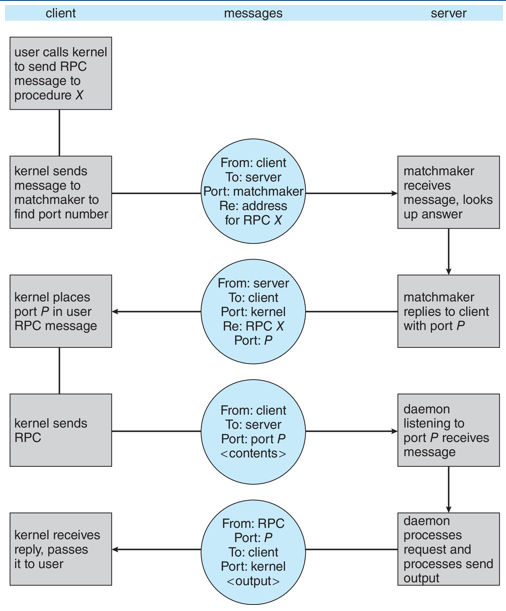
\includegraphics[width=0.7\linewidth]{img/RPC.png}
    \caption{Execution of RPC}
    
\end{figure}